% !TEX root = ./multilinear.tex

\section{Parallel algorithm: abstract description using a DAG representation}
\label{sec:proposed}

We describe our parallel algorithms in a more general form, for finding multilinear
terms in a multivariate polynomial, which can be represented as a DAG. 
Both problems \ref{prob:trees} and \ref{prob:macs} can be reduced to multilinear detection---this
follows from \cite{koutis:icalp08,williams2009finding} for problem \ref{prob:trees} and
from Section \ref{sec:scan-sequential} for problem \ref{prob:macs}. 
We note that the DAG representation
is only for the purpose of explaining the parallel algorithm for both these problems; we do not
solve the two problems by explicitly constructing DAGs. We will describe the specific algorithms
for both the problems by constructing the DAGs implcitly in Section \ref{sec:application}.

\subsection{Overview of the Algorithm}
We assume a DAG $G(V,E)$ which represents an instance of $k$-MLD, with levels
$\mathcal{L} = \{L_1,\ldots,L_{|\mathcal{L}|}\}$. The algorithm involves evaluating the
DAG in $2^k$ iterations, which are partitioned into ``phases'' of $N_2$ iterations each.
The idea is that a phase of $N_2$ iterations will be done simultaneously using $N_1$
processors. Let $N$ denote the total number of processors available. Therefore, $N/N_1$
phases can be done in parallel.

Let $N$ denote the total number
of processors available; of these $N_1$ will be used for each iteration. 
We assume the graph is partitioned into $N_1\leq N$ parts, denoted by
$\mathcal{P}=\{G^1= (V^1, E^1), \ldots, G^{N_1}=(V^{N_1}, E^{N_1})\}$; desirable properties of
the partition will be discussed later.
For each level $L_s\in\mathcal{L}$, let $L_s^j$ denote the corresponding level
in partition $j$; $\mathcal{L}^j$ denotes the set of all levels in that partition.
For level $L_s\in\mathcal{L}$, let $\maxload{}_s = \max_j |L_s^j|$ be the maximum
``load'' on partition $j$ from that level. Further, for $s<|\mathcal{L}|$, let
$\maxdeg{}_s = \max_{j\neq j'} |\{(u, v)\in L_s\times L_{s+1}: u\in L_s^j, v\in L_{s+1}^{j'}\}|$
denote the maximum number of edges from any $L_s^j$ to $L_{s+1}^{j'}$.
We will analyze the performance of our algorithm in terms of $\maxload{}_s$ 
and $\maxdeg{}_s$,
which motivates the properties of the partitioning to ensure best performance.

\begin{figure}[h]
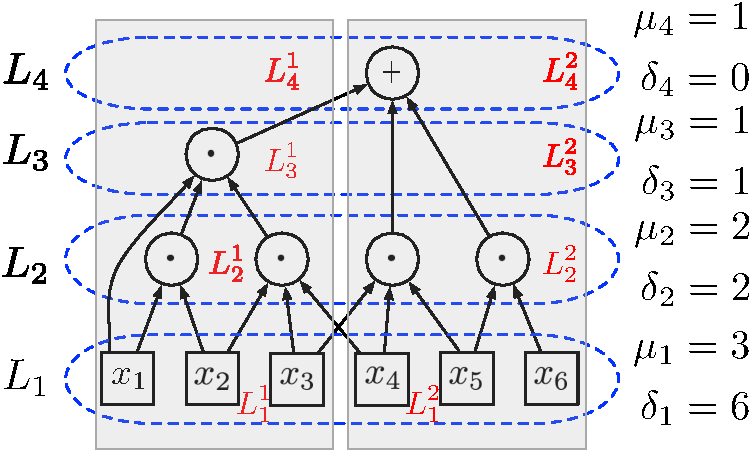
\includegraphics[width=0.4\textwidth]{img/dag4.pdf}
\caption{
\small
Illustration of the level sets and associated quantities for the DAG in
Figure \ref{fig:dag}, corresponding to a partition into two parts. 
%\vspace{-0.2in}
}
\label{fig:dag4}
\end{figure}

We describe the main intuition of the steps of Algorithm \parmaxwt{} below:
\begin{enumerate}
\item
The algorithm starts with the partitioning $\mathcal{P}$ of the graph $G$.
We discuss its complexity and implementation in Section \ref{sec:partition}.
\item
Each of the $2^k$ iterations in the while loop in lines 10-15 of \maxwt{}
is completely independent of others. Since $N_1$ processors are used for each iteration,
we run $\lfloor{N/N_1}\rfloor$ iterations in parallel, which require $\frac{2^k}{\lfloor{N/N_1}\rfloor}$
iterations of the while loop.
\item
Algorithm \parcircuit{} evaluates the circuit by levels, and computes
a value $\val(i)$ for each node $i$.
\item
For each node $i$ that we evaluate, we compute $\val(i)$ using the $\val(j)$ value for each predecessor $j$. 
If a predecessor $j$ is in the same partition $p'$, then, we can simply read $\val(j)$, 
as in the sequential algorithm. For every predecessor $j$ in a different partition, 
$j$ has to send a message with $\val(j)$, introducing a communication overhead.
\item
We aggregate the value at root$(G)$ over all $2^{k}$ iterations to get the final solution.
\end{enumerate}


\begin{algorithm}{}
\small
\caption{\parmaxwt{}$(G(V,E), k, \mathcal{L}, \epsilon, N_1, N_2)$.}
\label{alg:parallel-kMLD} 
\begin{algorithmic}[1]
\STATE \textbf{Input}: Circuit $G(V, E)$, parameter $k$, node levels $\mathcal{L}$,
confidence parameter $\epsilon\in (0, 1)$, parameters $N_1$ and $N_2$, which guide the parallelism.
\STATE\textbf{Output}: ``True" if circuit evaluation is non-zero. ``False" otherwise.

\STATE Let $v_i \in \mathbb{Z}_2^k$ be a random vector for each node $i$
\STATE Let $M = \bar 0$ be the polynomial
\STATE Let $N_1$ denote the number of processors used for each iteration.
Let $\mathcal{P}=\{G^1= (V^1, E^1), \ldots, G^{N_1}=(V^{N_1}, E^{N_1})\}$ denote the corresponding
partition of the graph into $N_1$ parts.
\STATE Let $a = \lfloor N / N_1 \rfloor$ be the number of iterations that will be run in parallel
\STATE Let count $=0$
\STATE \textbf{for} $\ell=1$ to $(\log{1/\epsilon})/(\log{5/4})$ 
\STATE \quad $M^{\ell}=0$
\STATE \quad \textbf{while} count$ < 2^k$ \textbf{do}
\STATE \quad \quad \textbf{for} $t =$ count$/N_2$ to $(\text{count} + a - 1)/N_2$ \textbf{do in parallel}
\STATE \quad \qquad  $M^{\ell}_{t,N_2} = \parcircuit(G(V, E), k, \mathcal{L}, \mathbf{v}, t, N_2, p, \mathcal{P})$
\STATE \quad \quad \textsc{MpiBarrier}
\STATE \quad \quad $M^{\ell} = M^{\ell} + \sum_{t=\text{count}/N_2}^{(\text{count} + a - 1)/N_2} M_{t,N_2} \mod 2^{k+1}$ using \textsc{MpiReduce}
\STATE \quad \quad count $= \text{count} + a$
\STATE \textbf{if} $M^{\ell}\neq 0$ for some $\ell$
\STATE \quad \textbf{return} \textbf{True}
\STATE \textbf{else} 
\STATE \quad \textbf{return} \textbf{False}
\end{algorithmic}
\end{algorithm}

\begin{algorithm}{}
\small
\caption{\parcircuit{$(G(V, E), k, \mathcal{L}, \mathbf{v}, t, p, \mathcal{P})$}}
\label{alg:parEvaluate} 
\begin{algorithmic}[1]
%\STATE \textbf{Procedure} \parcircuit{$(G(V, E), k, \mathcal{L}, \mathbf{v}, t, p)$}
\STATE \textbf{Input:} Circuit $G(V, E)$, parameter $k$, node levels $\mathcal{L}$, 
random assignment $\mathbf{v}$, iteration number $t$, number of partitions $p$, and
partitioning $\mathcal{P}$
%\STATE Partition $G$ into $p$ parts
%\STATE Let $G^{t,p'}$ be the partition assigned to processor $p'$
%\STATE Let $\mathcal{L}^{t,p'}$ be the corresponding levels assigned to processor $p'$
\STATE
\STATE \textbf{for} processor $p'$ \textbf{do in parallel}
\STATE \quad \textbf{Initialize circuit inputs}
\STATE \quad \textbf{for} node $i \in L^{p'}_{1}$ \textbf{do}
\STATE \qquad $ \val(i) = 1 + (-1)^{v_i^T \cdot t_{\text{bin}}}$

\STATE \quad \textbf{Evaluate the circuit by levels}
\STATE \quad \textbf{for} $s=2$ to $|\mathcal{L}^{p'}|$ \textbf{do}
\STATE \qquad \textbf{for} $i \in L_s^{p'}$ \textbf{do}
\STATE \qquad \quad \textbf{if} $\op(i) = +$ \textbf{then}
\STATE \qquad \qquad $\val(i) = \bar 0$
\STATE \qquad \qquad \textbf{for} $j \in \pred(i)\cap V^{p'}$ \textbf{do}
\STATE \qquad \qquad \quad $\val(i) = \val(i) + \val(j)$
\STATE \qquad \qquad \textbf{for} each incoming message $\langle j, \val(j)\rangle$ \textbf{do}
\STATE \qquad \qquad \quad $\val(i) = \val(i) + \val(j)$
\STATE \qquad \quad \textbf{else} 
\STATE \qquad \qquad $\val(i) = \bar 1$
\STATE \qquad \qquad \textbf{for} $j \in \pred(i)\cap V^{p'}$ \textbf{do}
\STATE \qquad \qquad \quad $\val(i) = \val(i) \cdot \val(j)$
\STATE \qquad \qquad \textbf{for} each incoming message $\langle j, \val(j)\rangle$ \textbf{do}
\STATE \qquad \qquad \quad $\val(i) = \val(i) \cdot \val(j)$
\STATE \qquad \quad  \textbf{Send result to successors in other processors}
\STATE \qquad \quad \textbf{for} $j \in \succ(i) \setminus V^{p'}$ \textbf{do}
\STATE \qquad \qquad \textbf{Send} $\langle i, \val(i)\rangle$
\STATE \textsc{MpiBarrier}
\STATE \textbf{return} $\val($root$(G))$
\end{algorithmic}
\end{algorithm}

Recall the definitions of $\maxload{}_s$ and $\maxdeg{}_s$ corresponding to the partitioning
$\mathcal{P}$ and corresponding level decomposition $\mathcal{L}^j, j=1,\ldots,p$.
Further, let $c_1$ and $c_2$ denote the time for unit computation at any node in $G$
and the unit communication along any edge, respectively, in the Algorithm \parcircuit{}.
The time and communication complexity of algorithm \parmaxwt{} is summarized below
in terms of these parameters.

\begin{theorem}
\label{thm:parmaxwt}
For any $\epsilon\in(0, 1)$,
Algorithm \parmaxwt{} solves the \textsc{$k$-MLD} problem for an
instance $P(x_1,\ldots,x_n)$ with probability at least $1-\epsilon$. The total time for
computation and communication are $O\left(c_1\frac{2^kp}{P}\sum_s \maxload{}_s\log{1/\epsilon}\right)$ 
and $O\left(c_2\frac{2^kp}{P}\sum_s \maxdeg{}_s\log{1/\epsilon}\right)$, respectively.
\end{theorem}
\begin{proof}
First, we argue the correctness.
For each value of $\ell$ in the outer for loop in lines 8-15 of Algorithm \parmaxwt{},
the while loop in lines 10--15 together correspond to the loop in lines 9--10
of the sequential algorithm \maxwt{} (since all the $2^k$ iterations are independent).
Therefore, the quantity $M^{\ell}$ computed in the lines 10--15 corresponds to the
result $M$ in line 12 of \maxwt{}. By Theorem \ref{theorem:kmld2}, if the
\textsc{$k$-MLD} instance $P(x_1,\ldots,x_n)$ has a multilinear term with $k$ variables,
then $\Pr[M^{\ell}\neq 0] = \frac{1}{5}$. This implies that if there is a multilinear term,
$\Pr[M^{\ell} = 0,\ \forall \ell] = (\frac{4}{5})^{(\log{1/\epsilon})/(\log{5/4})}\leq\epsilon$.

Next, we consider the computation and communication time complexity. 
The algorithm \parcircuit{} computes the DAG level by level within each iteration.
Therefore, the computation time for level $s\leq |\mathcal{L}|$ is 
$O(c_1\max_j |L_s^j|) = O(c_1\maxload{}_s)$, which is the maximum time for any processor
for this level. After this level is computed, the results have to be sent on all edges
in the set 
$\{(u, v)\in L_s\times L_{s+1}: u\in L_s^j, v\in L_{s+1}^{j'}\}$, for every pair of
processors $j, j'$. Therefore, the maximum communication time after level $s$ is
$\maxdeg{}_s = \max_{j\neq j'} |\{(u, v)\in L_s\times L_{s+1}: u\in L_s^j, v\in L_{s+1}^{j'}\}|$.
This implies the bounds on the total computation and communication steps.
\end{proof}

\subsection{Partition and Load Balancing}
\label{sec:partition}

From Theorem \ref{thm:parmaxwt}, the performance of Algorithm \parmaxwt{} depends crucially
on the partitioning. Specifically, the partition should be ``vertical'', i.e., one which achieves
load balance across each level and also minimizes the edge cut, which is formalized by
\[
\text{cost}(\mathcal{P}) = \sum_s (c_1\maxload{}_s + c_2\maxdeg{}_s)
\]

However, finding a partitioning $\mathcal{P}$ that minimizes the above objective
$\text{cost}(\mathcal{P})$ is NP-hard, in general, as summarized below. The proof
is omitted for brevity.

\begin{lemma}
\label{lemma:partition}
Given a DAG $G=(V, E)$ and per-unit computation and communication costs $c_1$ and $c_2$,
respectively, finding a partitioning $\mathcal{P}$ with the minimum cost is NP-hard, in general.
\end{lemma}

In light of Lemma \ref{lemma:partition}, we consider two heuristics: finding balanced
partitions in each level, and combining them, as well as METIS \cite{karypis:sijsc99}.

%We partition the circuit ``vertically"; that is, each processor gets a subset of nodes for each level in $\mathcal{L}$. Let $f(i)$ be the cost of evaluating node $v$. Then, we want to find a partition, such that
%$$
%\sum_{v \in V^p} f(i) \approx \frac{1}{p}\sum_{i \in V} f(i).
%$$

%\subsection{Analysis of Algorithm \parmaxwt{}}
%\subsubsection{Time Complexity}
%The \textbf{while} loop in lines 8--13 of \parmaxwt{} runs for at most $\frac{2^k}{P / p}$ iterations. For each iteration, each partition does work in the order $O(\frac{1}{p}\sum_{i \in V} f(i))$, so the total running time is $O(\frac{1}{p}(2^k f(V)))$.
%\subsubsection{Number of Messages}
%We assume that we have $P$ processors available and that $G$ does not fit in the memory of a single computing node. We have to use $p \leq P$ processors to store the graph in memory. We propose an MPI algorithm with roughly the following steps:

%\begin{enumerate}
%\item \parmaxwt{} Algorithm \ref{alg:parallel-kMLD}
%\item Determine $p$, the number of processors needed to store the graph.
%\item We have to run the loop from line 9 of \maxwt{}. Each of the $2^k$ iteration is independent of the others, so we can run $\lfloor{P/p}\rfloor$ iterations in parallel.
%\item \parcircuit{} Algorithm \ref{alg:parEvaluate}
%\item For each iteration $t$, we first partition the circuit into $p$ parts, and we evaluate these parts in parallel.
%\item For each partition $p'$, we evaluate the circuit by levels, as in \maxwt{}. 
%\item For each node $i$ that we evaluate, we compute $m(i)$ using the $m(j)$ value for each predecessor $j$. if a predecessor $j$ is in the same partition $p'$, then, we can simply read $m(j)$, as in the sequential algorithm. For every predecessor $j$ in a different partition, $j$ has to send a message with $m(j)$, introducing a communication overhead.
%\item We aggregate the value at root$(G)$ over all $2^{k}$ iterations to get the final solution.
%\end{enumerate}

%\noindent
%\textbf{Algorithm \ref{alg:parallel-kMLD}}: \parmaxwt{}\\
%1. Determine $p$, the number of processors needed to store the graph.\\
%2. We have to run the loop from line 9 of \maxwt{}. Each of the $2^k$ iteration is independent of the others, so we can run $\lfloor{P/p}\rfloor$ iterations in parallel.\\
%\textbf{Algorithm \ref{alg:parEvaluate}}: \parcircuit{} \\
%3. For each iteration $t$, we first partition the circuit into $p$ parts, and we evaluate these parts in parallel.\\
%4. For each partition $p'$, we evaluate the circuit by levels, as in \maxwt{}. \\
%5. For each node $i$ that we evaluate, we compute $m(i)$ using the $m(j)$ value for each predecessor $j$. If a predecessor $j$ is in the same partition $p'$, then, we can simply read $m(j)$, as in the sequential algorithm. For every predecessor $j$ in a different partition, $j$ has to send a message with $m(j)$, introducing a communication overhead.\\
%6. We aggregate the value at root$(G)$ over all $2^{k}$ iterations to get the final solution.
